\section{پاسخ.}

	\begin{redtext}
	در این حالت، فرض می‌کنیم که $\mathcal{S}$ مجموعه نمونه‌ها باشد، بطوری که:
		\begin{equation*}
			\mathcal{S} = ((x_1, y_1), \dots, (x_m, y_m)), \quad\quad x_i \in \mathbb{R}^d, \quad y_i \in \mathbb{R}^p
		\end{equation*}
	که در این‌جا، $d$ و $p$ به ترتیب ابعاد فضای ویژگی و فضای برچسب هستند. همان‌طور که مشاهده می‌کنید، در این حالت فضای برچسب (خروجی) $p$ بُعدی است، یعنی به ازای هر نمونه، به تعداد $p$ برچسب در اختیار داریم. حال برای حل چنین مسئله‌ای، می‌توان از دو رویکرد کلی استفاده کرد که در ادامه آن‌ها را شرح خواهیم داد.
		
		\subsection*{روش اول: رگرسیون چند خروجی مستقیم.}
			یکی از ساده‌ترین رویکردهای قابل ارائه برای حل چنین مسئله‌ای، استفاده از رگرسیون چند خروجی مستقیم\LTRfootnote{Direct Multioutput Regression} است. در این سناریو، به ازای هر بُعد از فضای برچسب، یک مدل رگرسیون ساخته می‌شود که روی مجموعه داده $\mathcal{X}$ آموزش می‌بیند (شکل \ref{fig2}). بنابراین باتوجه به فضای ویژگی $\mathcal{X}$ که برابرست با:
			\begin{equation*}
				\mathcal{X} = (x_1, \dots, x_m), \quad\quad x_i \in \mathbb{R}^d
			\end{equation*}
			یک مجموعه از فرضیه‌ها با نام $\mathcal{\hat{H}}$ در اختیار داریم، به‌طوری که:
			\begin{equation*}
				\mathcal{\hat{H}} = \big\{ \phi: \mathcal{X} \times \Theta \rightarrow \mathbb{R} \big\}, \quad\quad | \mathcal{\hat{H}} | = p
			\end{equation*}
			که در این مجموعه، $\phi_i$ مدل $i$-ام برای تخمین بًعد $i$-ام فضای برچسب‌ها است.
			
			\begin{figure}[h]
				\centering
				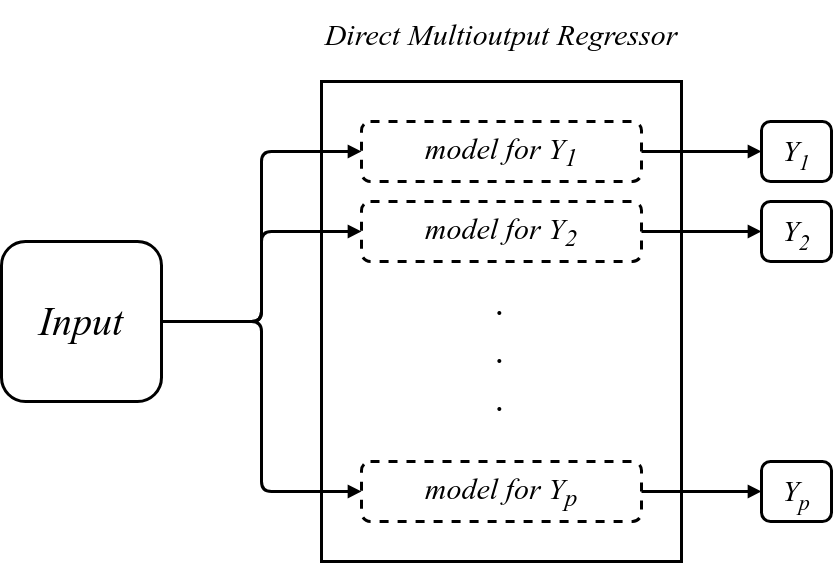
\includegraphics[width=8cm, height=4.5cm]{direct_mulit-output_reg.png}
				\caption{معماری کلی یک رگرسیون چند خروجی مستقیم.}
				\label{fig2}
			\end{figure}
		
		\subsection*{روش دوم: رگرسیون چندخروجی زنجیره‌ای.}
		در این معماری، مدل‌ها به صورت زنجیره‌ای و پشت سرهم ساخته می‌شوند، به‌طوری که هر مدل با استفاده از فضای ویژگی $\mathcal{X}$ و پیش‌بینی مدل قبل آموزش می‌بیند. به چنین روشی، رگرسیون چندخروجی زنجیره‌ای\LTRfootnote{Chained Multioutput Regression} گوییم. این روش در مسائلی که ابعاد خروجی از نظر مفهومی با یکدیگر مرتبط هستند می‌تواند کارا باشد. بنابراین در این روش نیز مجموعه‌ای از فرضیه‌ها با نام $\mathcal{\hat{H}}$ در اختیار داریم، به‌طوری که:
		\begin{equation*}
			\mathcal{\hat{H}} = \big\{ (\forall_{0 \leq i \leq p}) \phi_i: \mathcal{X} \times Y_{i-1}\times \Theta_i \rightarrow \mathbb{R} \big\}, \quad\quad | \mathcal{\hat{H}} | = p
		\end{equation*}
		بنابراین آخرین مدل در این معماری، فضای ویژگی‌ای با ابعاد $d + p - 1$ در اختیار دارد که این خاصیت در این معماری، می‌تواند به تدریج تأثیر مدل‌های قبلی را دریافت کند. البته این خاصیت می‌تواند جز معایب این روش نیز باشد. اگر مدل‌های آغازین عملکرد خوبی در پیش‌بینی برچسب متناظرشان نداشته باشند، آن‌وقت به تدریج مدل‌های آخر فضای ویژگی‌شان دارای ویژگی‌های غیرمفید می‌شود و از نظر محاسباتی نیز هزینه بیشتری دربردارد.
		
		\begin{figure}[h]
			\centering
			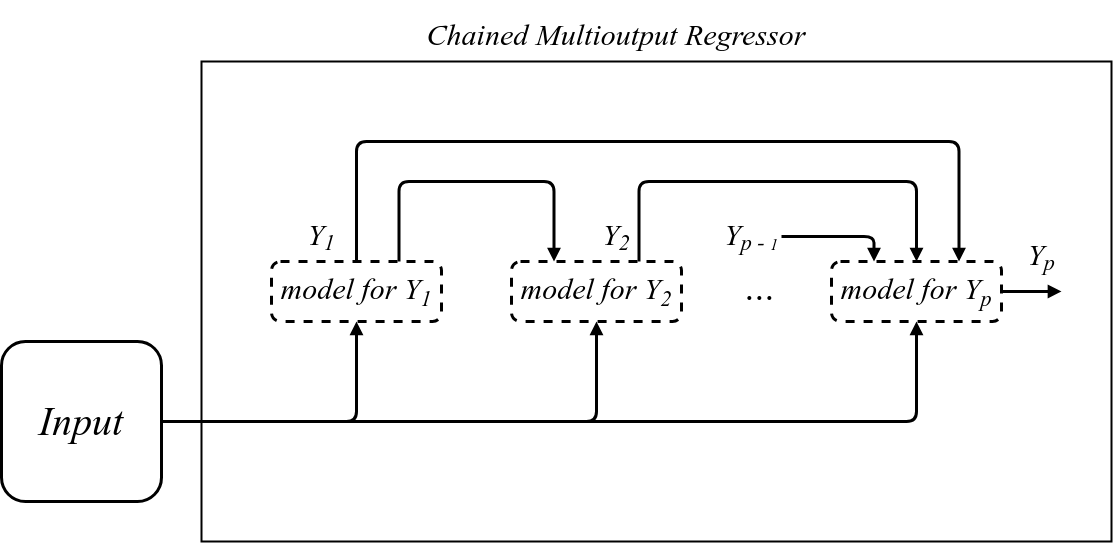
\includegraphics[width=12cm, height=6cm]{chained_multi-output_regression.png}
			\caption{معماری کلی یک رگرسیون چند خروجی زنجیره‌ای.}
			\label{fig3}
		\end{figure}		
		
	\end{redtext}


